\chapter{Introduction}
%labels will help you to reference to certain images, tables, chapters, section, and so on...
\label{introduction}
%DELETEME: for readability purpose, it makes sense to write a short paragraph on what the reader can expect in this chapter.

%DELETEME: tipp: sometimes it makes sense to write the first chapter, the last chapter, and the abstracts at the end. In this case, it might be easier to argue towards your topic


%###################################################################################
%###################### Motivation          ########################################
%###################################################################################


\chapter{Motivation}

Autonomous systems continue to improve at specialized tasks allowing for a higher quality of life for many individuals. Intelligent robotics have historically assumed tasks that would otherwise be arduous, vacuous, or even dangerous for humans. Specifically designed for distinct tasks, these machines do not grow tired over time and have efficiency/accuracy rates not typically achievable by humans (i.e., the manufacturing of vehicles or throughput of products on an assembly line). However, these topics are usually 'behind the scenes', as little-to-no human interaction is required. Recently, autonomous systems are proposed to coalesce and proliferate everyday activities via autonomous driving, product distribution, and tasks that require repetitive actions that do not require critical thinking. 
\smallskip

Throughout the world, safety is a major concern for people and is a major factor of \textit{Quality of Life} (QoL). In Germany alone, 23\% of urban denizens report feeling unsafe due to crime in 2016 (\cite{eurostat}). As such, there is a major need for improving the QoL for citizens, especially in urban areas. In general, police forces are responsible for the reduction of crime. Special forces units are called in whenever there are high-profile missions containing dangerous criminals (homicides, hostage situations, counterterrorism, etc.). In these situations, there is a high level of risk for the operatives that can result in permanent physical/mental damage or death. Another complication is that these operatives must wear additional protective gear. This gear blocks their ability to function ideally, as the total weight of gear can be upwards of 50kg and helmets/flak jackets block mobility. To combat these limitations, mixed human-robot teams can be assembled, sending in robots in to assess certain dangers (reconnaissance), structural damage, and even first contact with the perpetrator. 
\smallskip


While certain aspects of autonomous systems currently prevent their abundance in urban environments (privacy concerns, resources, technological feasibility, etc.), there are additional niche areas that can immediately benefit from mixed human-robot teams for safety outside of police work. These stakeholders/areas/events include firefighters, disaster relief, item retrieval, contraband/explosives disarmament, and other environments in which the presence of a robot would reduce the risk of danger for human operators. In terms of interoperability and scalability, human-robot system design should find commonalities between these types of events and create a standardized framework.
\smallskip

Within the fields of autonomous systems and human-robot interaction, there is a lot of work to be completed. In the case of mixed human-robot teams, proper perception/cognition (for the robot) and distance (\textit{Personal-Space Model}) for the user (\cite{cuijpers}) is being analyzed with parametric models based on commonalities in user experience and comfort. Decision-making operations are currently in development for autonomous agents for reactive-adaptive hybrid behavior-based planning (\textit{ROS Hybrid Behavior Planner} RHBP)  (\cite{hrabia1}). In fact, simple navigation and interaction with robots is not a trivial task that cannot be solved solely with intuition. 
\smallskip

\section{Project Scope}
This project will be in direct relation to the needs of the Brandenburg  \textit{Spezialeinsatzkommandos} (SEK) (EN: Special Deployment Commandos), a German Special Forces group (Fig. \ref{sek}). Their operations are often conducted in small, indoor environments where mobility and visibility are limited. As a special operation, counter-terrorism, and high-risk unit, they deal with the most critical tasks including hostage sieges, building raids, and surveillance (\cite{SEK1}). Adding \textit{Unmanned Aerial Vehicles} (UAVs) to their teams allows for a unique opportunity to minimize the danger of field operators during their missions. While certain military groups, like the \textit{United States Marine Corps} (USMC), have been experimenting with drones (DE: Drohne) during operations, these have largely been outdoors and a safe distance from the target (Fig. \ref{usmc})(\cite{USMC1}). This project will have additional challenges in which the drone acts as a support member in a mixed human-robot team, providing information on target identification/classification, environmental hazards (smoke, fire), and structural layout. 
\smallskip


\begin{figure}[htb]
\centering
\makebox[\textwidth]{
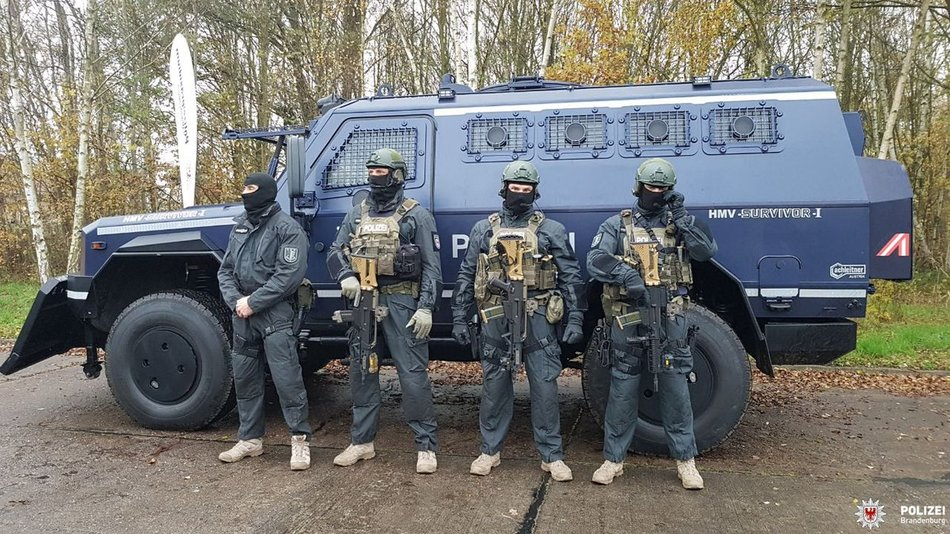
\includegraphics[width = .95\textwidth]{gfx/sek.jpg}}\\
\caption{\label{sek}{Image of the Brandenburg SEK Force. Tactical gear prioritizes safety which negatively impacts vision, mobility, and cognitive load (\cite{BradSEK}). }}
\end{figure}
\bigskip



\begin{figure}[htb]
\centering
\makebox[\textwidth]{
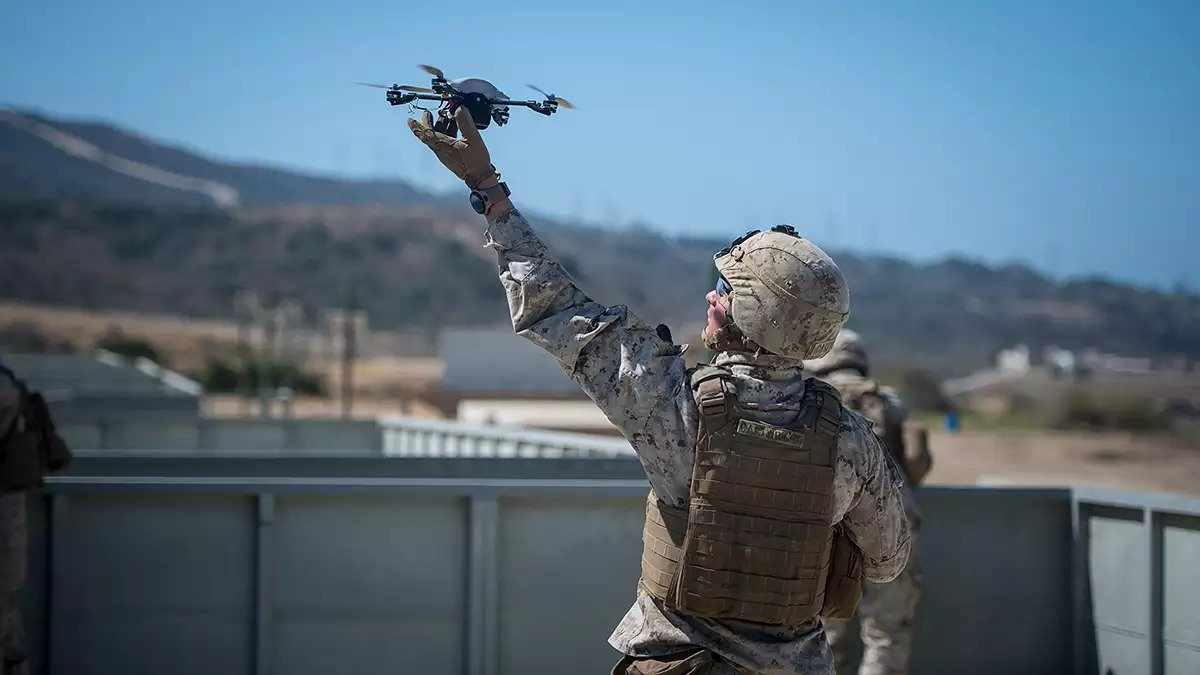
\includegraphics[width = .95\textwidth]{gfx/003.jpg}}\\
\caption{\label{usmc}{Image of USMC operative with a drone (\cite{USMC1}). }}
\end{figure}


\newpage







%\section{Motivation}
%DELETEME: This section is very important since it argues why it is necessary to take care of the problem you are addressing in your work. One way to do this is coming from a very broad view on the problem to a very detailled one. This can be done by establishing a chain of statements that refer to each other until you reach your particular problem. Doing this, you really need to take care for citing every statement. 

%DELETEME: Example for a chain: Mobile communication gets increasingly popular in the world (CITE sales on mobile communication infrastruce, mobile phones, or increasing number of mobile phones contracts). $\rightarrow$ Especially smartphones, which represent the next generation cellular phone (CITE), get more and more used for communicating not only with other people but also for connecting to the Internet for using various services (CITE). $\rightarrow$ Smartphone are comprehensive cellular phones that provide additional functionality due to their increased connection and processing capabilities (CITE). $\rightarrow$ Most smartphones offer an online application store for adding software to the devices which helps the users to customize their devices according to their needs, e.g. Android Market\footnote{\url{http://market.android.com}, visited on 05/08/2011}. $\rightarrow$ One problem about installing third-party software is that not all softwares try to help the user; $\rightarrow$ software with malicious intentions, so called malicious software (malware), can be a severe threat to smarpthone users. Some malwares delete files (EXAMPLE + CITE or footnote with URL) or even destroy devices (EXAMPLE + CITE or footnote with URL). $\rightarrow$ More and more smartphone malwares appeared in the last years (CITE). $\rightarrow$ Signature-based approaches work efficiently on known malware (CITE) but face serious drawbacks regarding unknown malware. $\rightarrow$ Oberheide et al.~\cite{oberheide:2008:cloudav} state that virus engines need an average time of 48 days until their databases get updated to be able to detect a certain unknown malware. $\rightarrow$ This in turn means that smartphone users stay unprotected for this time which can be seen as a severe threat. $\rightarrow$ Therefore, approaches are needed that are capable of detecting unknown malware for protecting the users against such threats.
%DELETEME: This example showed how one could argue that alternative approaches for malware detection is required. The length of the motivation depends on the topics handled and can of course be longer. The principle I am describing is also shown on Figure~\ref{fig:writing}

%\begin{figure}
%\centering
%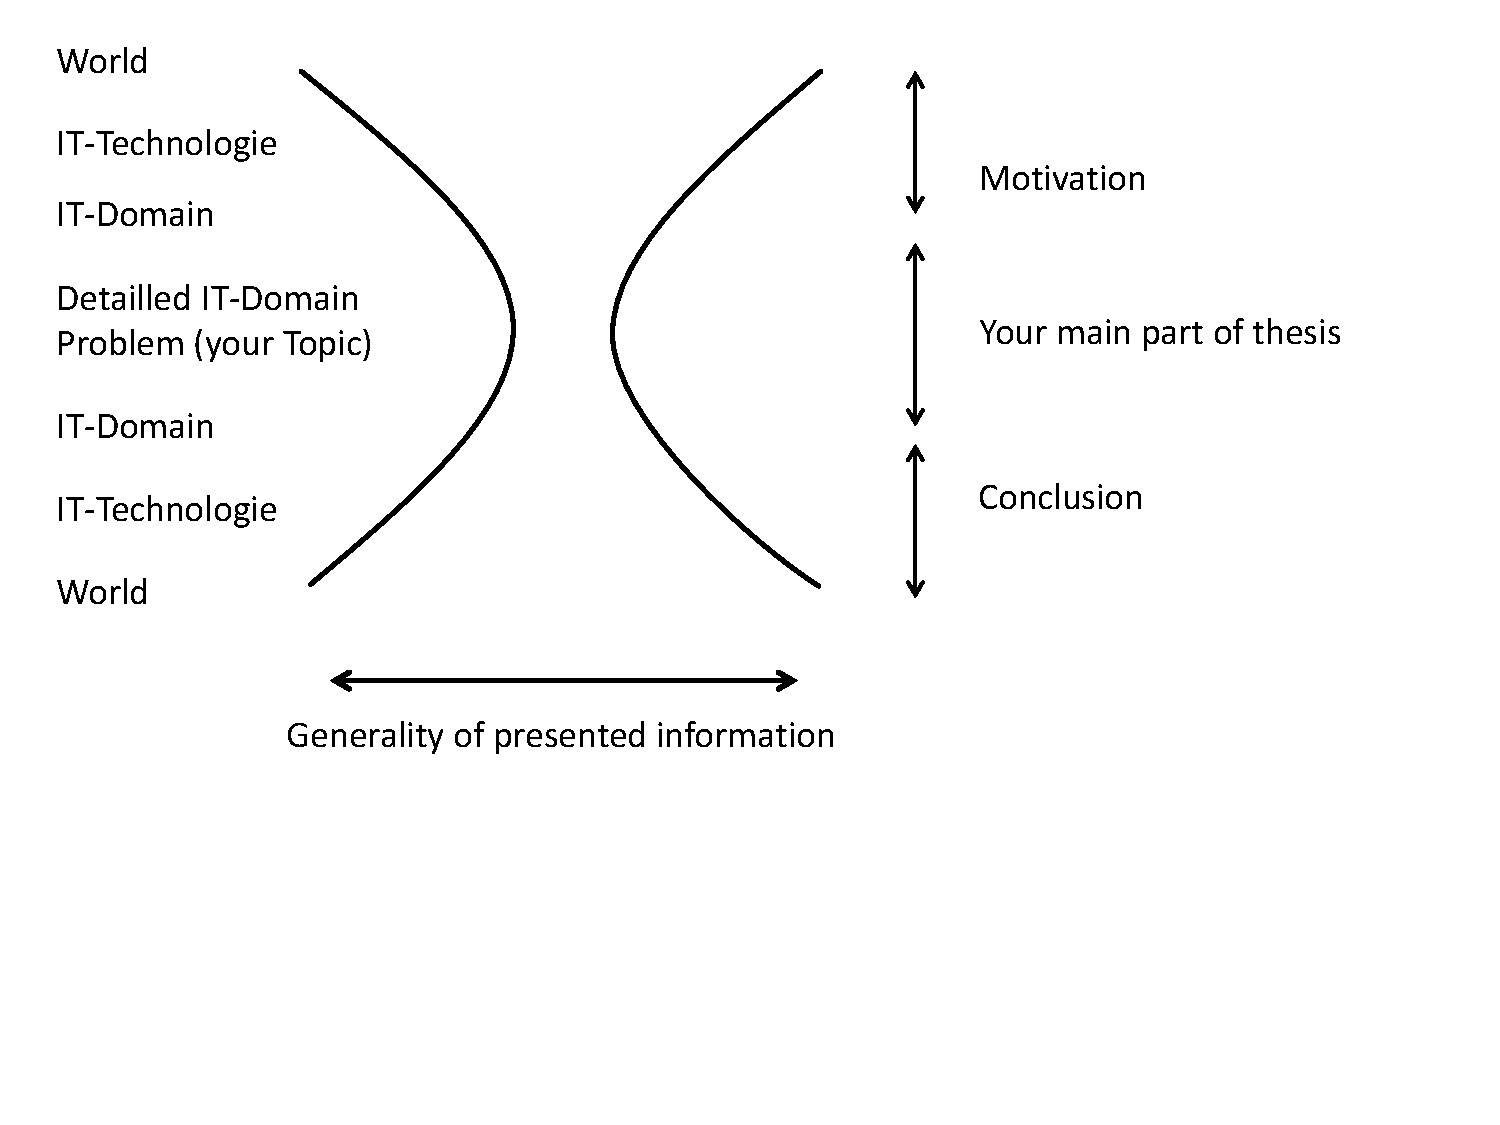
\includegraphics[width=0.9\textwidth]{template/writing}
%\caption[Information Generality]{This images illustrates how generality of information could be handled in a thesis. In your motivation you should start from a very broad view on the topic. Then you should get more precise with every statement until you reach the actual problem you are addressing. You should do vice-versa in your conclusion, starting with the problem that you addressed and getting broader until you can write about the meaning of your results to the (IT-)world.\label{fig:writing}}
%\end{figure}


%###################################################################################
%###################### Approach and Goals  ########################################
%###################################################################################
%\section{Approach and Goals}
%DELETEME: In this section, you should cleary describe your approach that you are following in order to solve the underlaying problem of your thesis. Additionally, you should clearly state the goals of your work. This will not only help you supervizor to understand what you are doing, it will also help you to be sure on which topic you should evaluate.


%###################################################################################
%###################### Structure of the Thesis ####################################
%###################################################################################
%\section{Structure of the Thesis}
%DELETEME: This section does not require eloquent writing. It is just a presentation of what you will handle in each chapter starting with Chapter~\ref{background}.

%DELETEME: Example: This thesis is structured as follows. In Chapter~\ref{background}, we discuss essential background related to the thesis topic. (SOME MORE SENTENCES). Chapter~\ref{mainone} represents a detailled analysis of the problem that will be addressed. In particular, (SOME MORE SENTENCES). In Chapter~\ref{maintwo}, our solution is presented. This solution covers ... (SOME MORE SENTENCES). Chapter~\ref{evaluation} evaluates our solution basing on our specified goals. (SOME MORE SENTENCES). In Chapter~\ref{conclusion}, we conclude. Chapter~\ref{appendices} gives additional related information on the topic of this thesis.